\documentclass[svgnames,9pt]{beamer}
%\usepackage[latin1]{inputenc}
\usepackage{ragged2e}
\usetheme{Warsaw}
\setbeamertemplate{headline}{}
\setbeamerfont{footline}{size=\fontsize{6}{8}\selectfont}
\makeatletter
\expandafter\def\expandafter\insertshorttitle\expandafter{%
	\insertshorttitle\hfill%
	\insertframenumber\,/\,\inserttotalframenumber}
\setbeamertemplate{frametitle}
{%
	
	\nointerlineskip%
	\vskip-2pt%
	\hbox{\leavevmode
		\advance\beamer@leftmargin by 12bp%
		\advance\beamer@rightmargin by 12bp%
		\beamer@tempdim=\textwidth%
		\advance\beamer@tempdim by \beamer@leftmargin%
		\advance\beamer@tempdim by \beamer@rightmargin%
		\hskip-\Gm@lmargin\hbox{%
			\setbox\beamer@tempbox=\hbox{\begin{minipage}[b]{\paperwidth}%
					\vbox{}\vskip.50ex% NEW: original \vskip-.75ex
					\leftskip0.3cm%
					\rightskip0.3cm plus1fil\leavevmode
					\insertframetitle%
					\ifx\insertframesubtitle\@empty%
					\strut\par%
					\else
					\par{\usebeamerfont*{framesubtitle}{\usebeamercolor[fg]{framesubtitle}\insertframesubtitle}\strut\par\vskip2ex}% NEW: added \vskip2ex
					\fi%
					\nointerlineskip
					\vbox{}%
			\end{minipage}}%
			\beamer@tempdim=\ht\beamer@tempbox%
			\advance\beamer@tempdim by 2pt%
			\begin{pgfpicture}{0pt}{0pt}{\paperwidth}{\beamer@tempdim}
				\usebeamercolor{frametitle right}
				\pgfpathrectangle{\pgfpointorigin}{\pgfpoint{\paperwidth}{\beamer@tempdim}}
				\pgfusepath{clip}
				\pgftext[left,base]{\pgfuseshading{beamer@frametitleshade}}
			\end{pgfpicture}
			\hskip-\paperwidth%
			\box\beamer@tempbox%
		}%
		\hskip-\Gm@rmargin%
	}%
	\nointerlineskip
	\vskip-0.2pt
	\hbox to\textwidth{\hskip-\Gm@lmargin\pgfuseshading{beamer@topshade}\hskip-\Gm@rmargin}
	\vskip-2pt
}
\makeatother
\addtobeamertemplate{frametitle}{\vspace*{0.5cm}}{\vspace*{0.5cm}}

\title[Handwritten Digit Recognition Using Improved Bounding Box Recognition Technique]{\huge \textbf{Python coding for geospatial processing in web-based mapping applications}  } %Project title
\author[Group-14]{}

\date{}

\begin{document}
	\begin{frame}
		
		\begin{figure}[h!]
			
\includegraphics[scale=0.5]{stthomaskannur.png}
		\end{figure}
		
		\begin{center}      
			\begin{minipage}[b]{1.0\textwidth}
				\centering
				Department of Computer Science and Engineering\\
				St. Thomas College of Engineering and Technology\\Mattannur
			\end{minipage}%
		\end{center}
		
		\titlepage
		
		\begin{minipage}[t]{0.5\textwidth}
			\vspace{-2cm}
			\begin{flushleft}
				{ \textit{Author}:\vspace*{0.1cm} \\ ARPIT RAMESAN (STM19CS017)\\ JEREESH ISMAIL C K (STM19CS024)\\ VAISHNAVI RAJEEVAN (STM19CS057) } %students name
			\end{flushleft}
		\end{minipage}%
		%
		\begin{minipage}[t]{0.5\textwidth}
			\vspace{-2cm}
			\begin{flushright}
				{\textit{Supervisor}:\vspace*{0.1cm} \\ MR.JITHIN S} %supervisor name
			\end{flushright}    
		\end{minipage}%
		
		\vspace{-0.7cm}
		\begin{center}      
			\begin{minipage}[b]{0.5\textwidth}
				\centering  
				\small Academic Year \\ 2021-22\\ \today
			\end{minipage}%
		\end{center}    
	\end{frame}
\section{OUTLINE}
\begin{frame}{OUTLINE}
        \tableofcontents
\end{frame}
\section{INTRODUCTION}
\begin{frame}{INTRODUCTION}
\begin{itemize}
\justifying \item Web based mapping applications are effective in providing
simple and accessible interfaces for geospatial information,
and often include large spatial databases and advanced analytical capabilities. 
\item Perhaps the most familiar is Google Maps [Ggl] which provides access to terabytes of maps,
aerial imagery, street address data, and p2p routing
capabilities. 
\item Descriptions are included herein of several Web based applications that focus on energy and environmental data
and how their back end geoprocessing services were built with
Python.
\end{itemize}
\end{frame}

\section{PROBLEM IDENTIFICATION}
\begin{frame}{PROBLEM IDENTIFICATION}
\begin{itemize}
\justifying \item In today's world there is a lot of issues regarding proper navigation at a much efficient and cost affordable manner. 
\item That is,the usage of maps in our daily lives may cost a lot of data and a big data usage for storage.
\item So by using libraries that are built with Python ArcGIS, we are able to build a mapping system that helps us to provide the same mapping system but at a more improved and efficient manner.
\item Hence the work done is completely based on Web based tools that is available for all.
\end{itemize}
\end{frame}

\section{LITERATURE SURVEY}
\begin{frame}{LITERATURE SURVEY 1}
\textbf{A non-GPS based location tracking of public buses using Bluetooth proximity beacons}
\begin{itemize} 
\justifying \item Tracking of public bus location requires a GPS device to be installed and many bus operators in developing countries do not have such a solution in place provide an accurate estimation of bus arrival (ETA).
\item Without ETA info, it is very difficult for the general public to plan their journey effectively. 
\item This paper proposes an innovative IoT solution to track the location of buses without requiring the deployment of GPS device. 
\item It uses Bluetooth Low Energy(BLE) proximity beacon to track the journey of a bus by deploying an estimate location beacon on the bus.
\end{itemize}
\end{frame}
\begin{frame}{LITERATURE SURVEY 2}
\textbf{Double lane line edge detection method based on constraint condition Hough Transform}
\begin{itemize}
\justifying \item The proposed lane detection method is based on Hough Transform double edge extraction. 
\item This lane line detection method is used in many self driving autonomous vehicles as well as line following robots.
\item There are two kinds of lane line detection methods proposed by scholars at home and abroad: Model based and feature based.
\item For the straight lane line, the Hough Transform based on polar angle an  polar radius constraints is used to obtain the double edges of lane lines and straight line points are used to determine the end points and starting points of straight lane lines to complete straight line fitting.
\end{frame}
\begin{frame}{LITERATURE SURVEY 2(Cont...)} 
\textbf{EXISTING SYSTEM} 
\begin{itemize} 
\justifying \item The current system used for navigation includes usage of high amounts of data and usage of a lot of storage space.
\item Apart from that, there exists various model websites which showcase the ArcGIS framework on a public level. But it is only available as a paid tool.
\item Also this model works in a complex manner and hence has trouble in implementation as it requires subject knowledge for the same. 
\item There are multiple web-based applications that provide the necessary resources for building the structure for geospatial mapping using python.
\end{itemize}
\end{frame} 
\section{PROPOSED SYSTEM DESIGN} 
\begin{frame}{PROPOSED SYSTEM DESIGN}
\begin{itemize}
\justifying \item To build a website that acts as a host for geospatial mapping using the ArcGIS framework.
\item The system would be able to display the current location and destination locations of the user and provide a map for the same.
\item The proposed system is completely based on the ArcGIS framework and will be implemented as a website using the Jupyter python library for code development.
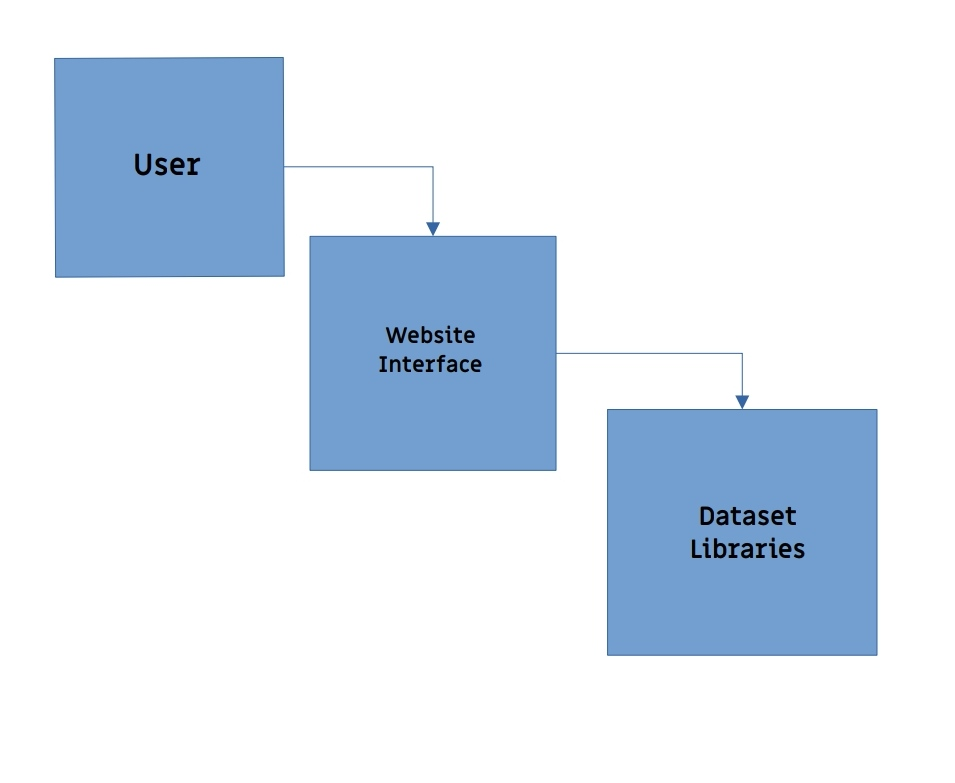
\includegraphics[scale=1.5]{archi.jpg}
\end{itemize@}
\end{frame} 
\section{CONCLUSION}
\begin{frame}{ CONCLUSION }     
\begin{itemize}
\justifying \item Python is the de facto standard scripting language in both
the open source and proprietary GIS world. 
\item Most, if not all,
of the major GIS software systems provide Python libraries
for system integration, analysis, and automation, including
ArcGIS, GeoPandas [GeoP], geoDjango [geoD], GeoServer,
GRASS, PostGIS, pySAL [pySAL], and Shapely [Shp]. 
\item Some of these systems, such as ArcGIS and geoDJango, provide
frameworks for web based mapping applications different
from the approach  we had mentioned. 
\item All examples are written in Python and run within the OGC-compliant WPS framework provided by PyWPS.
\end{itemize}
\end{frame}
\section{REFERENCES}
\begin{frame}{REFERENCES}
\begin{thebibliography}{99}
\justifying \bibitem{Tools}  Argonne National Laboratory, Energy Zones Study: A Comprehensive Web Based Mapping Tool to Identify and Analyze Clean EnergyZones in the Eastern Interconnection, ANL/DIS 13/09, September2013. Available at 
\url{https://eispctools.anl.gov/document/21/file} 
\bibitem{Locations}  \url{http://getbootstrap.com} 
{U.S. Department of the Interior, Bureau of Land Management,and U.S. Department of Energy, Final Programmatic EnvironmentalImpact Statement for Solar Energy Development in Six SouthwesternStates, FES 12-24, DOE/EIS-0403, July 2012. Available at} \url{http://solareis.anl.gov/documents/fpeis} 
 Kuiper, J., Ames, D., Koehler, D., Lee, R., and Quinby, T., webBased Mapping Applications for Solar Energy Project Planning inProceedings of the American Solar Energy Society, Solar 2013 Conference.
\end{thebibliography}
\end{frame} 
\end{document}
